\subsubsection{\texttt{RF-3}: seguimiento en tiempo real de progreso de ejercicios}
\label{subsec:rf3}

Cuando utilizan la extensión para Visual Studio Code, los docentes disponen de la capacidad para visualizar el \textit{dashboard} de un ejercicio, que muestra métricas actualizadas en tiempo real sobre el progreso de los estudiantes. Del mismo modo, la extensión incorpora una pantalla muy parecida que permite realizar un seguimiento en tiempo real sobre cada ejercicio de los cursos impartidos por un docente.

\begin{figure}[ht]
    \centering
    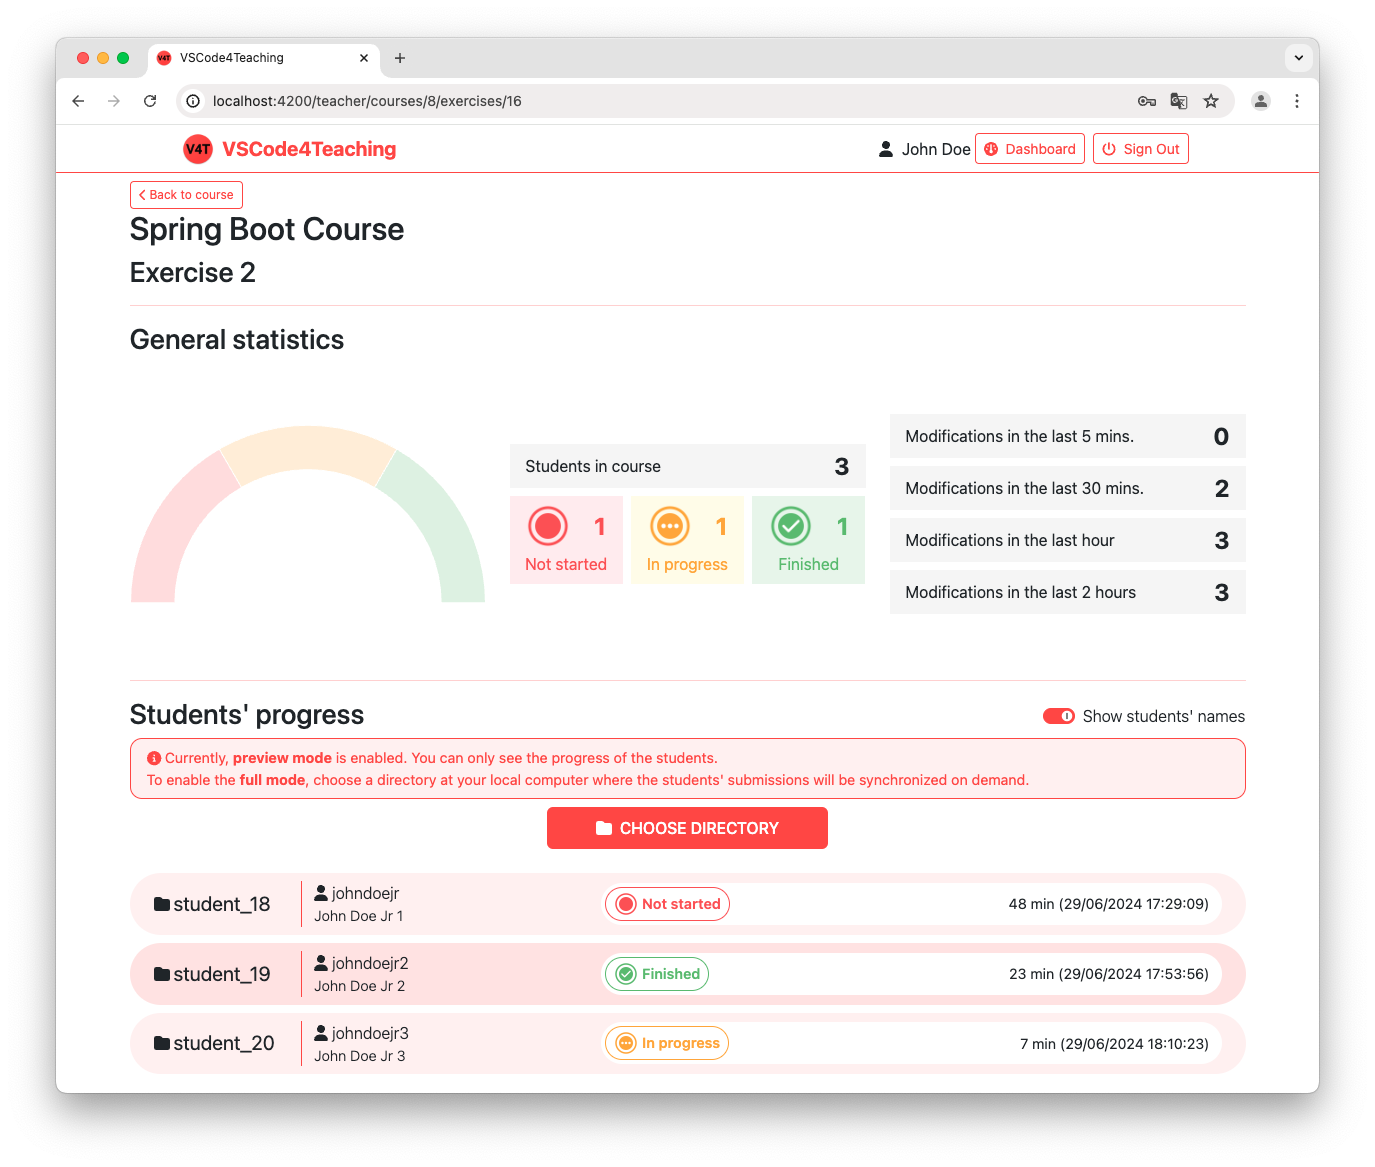
\includegraphics[width=\textwidth]{imagenes/utilizadas/4-3-implementacion/rf3-1.png}
    \caption{\textit{Dashboard} de un ejercicio en la aplicación web con métricas actualizadas en tiempo real para el seguimiento del progreso de los estudiantes.}
    \label{fig:reqf3-1}
\end{figure}

Se incluye una captura de esta visualización en la \referenciaFigura{fig:reqf3-1}. Esta visualización permite ver a los docentes rápidamente cuántos estudiantes hay matriculados en el curso ---y, por tanto, cuántos alumnos realizarán potencialmente el ejercicio---, desgranados debajo según el progreso, diferenciando los que no lo han iniciado, los que están realizándolo y los que lo han finalizado, incluyendo una gráfica semicircular representativa adyacente. Además, también se muestra cuántos estudiantes han modificado su propuesta en los últimos cinco y treinta minutos, en la última hora y dos horas. Debajo de estas estadísticas generales, es posible visualizar el progreso individualizado de cada estudiante, que se muestra de forma anónima: junto a cada directorio de cada propuesta de resolución aparecen el estado del ejercicio y la fecha y tiempo transcurrido tras la última modificación. Es posible asociar cada propuesta de resolución a su autor al modificar el control ``Show students' names'', lo que hará que se muestre en cada fila, además, el apodo y nombre completo de cada estudiante.

La extensión permite disponer del \textit{dashboard} en dos formatos: en forma de previsualización, mostrando únicamente las métricas anteriormente relatadas, o en formato completo, permitiendo abrir los ficheros que componen la propuesta de cada estudiante. Análogamente, la aplicación web permite visualizar únicamente las métricas en formato de previsualización y, además, da al docente la opción de escoger un directorio local para descargar en él bajo demanda las distintas propuestas de los estudiantes, tal como se detalla en el requisito \referenciaConTT{subsec:rf4}{RF-4}.
